\documentclass[a5paper]{article}
\usepackage[a5paper, top=17mm, bottom=17mm, left=17mm, right=17mm]{geometry}
\usepackage[utf8]{inputenc}
\usepackage[T2A,T1]{fontenc}
\usepackage[colorlinks,filecolor=blue,citecolor=green,unicode,pdftex]{hyperref}
\usepackage{cmap}
\usepackage[english,russian]{babel}
\usepackage{amsmath}
\usepackage{amssymb,amsfonts,textcomp}
\usepackage{color}
\usepackage{array}
\usepackage{hhline}
\hypersetup{colorlinks=true, linkcolor=blue, citecolor=blue, filecolor=blue, urlcolor=blue, pdftitle=1, pdfauthor=, pdfsubject=, pdfkeywords=}
\usepackage{graphicx}
\usepackage{indentfirst}
\usepackage{wrapfig}

\sloppy
\pagestyle{plain}

\title{Студенческие проекты по программированию как средство формирования профессиональных навыков}

\author{Т.А.Брыксин \\ timofey.bryksin at gmail dot com}
\date{}
\begin{document}


\maketitle
\thispagestyle{empty}


\renewcommand{\thefootnote}{}
%% ***************************************************************************
%% **                                                                       **
%% ** Авторские права                                                       **
%% **                                                                       **
%% ***************************************************************************
\footnote{\small{\copyright~Т.А.Брыксин, ~2011.}}
\renewcommand{\thefootnote}{\arabic{footnote}}
\setcounter{footnote}{0}



\begin{quote}
\small\noindent
В статье рассматривается проблема формирования практических навыков у студентов университетов, обучающихся по IT-специальностям. Обсуждается идея организации студенческих проектов и летних школ по программированию как средства сближения классического университетского образования и индустрии. Приводится обзор и анализ летних школ и студенческих проектов, проводившихся на базе кафедры системного программирования СПбГУ, обсуждаются трудности в организации подобных мероприятий.
\end{quote}

{\bf Ключевые слова:} программная инженерия, обучение программной инженерии.


\section*{Введение} 
Программная инженерия (software engineering,~\cite{swebok}) -- это сравнительно молодая и динамично развивающаяся область знаний. В условиях непрерывной эволюции аппаратных платформ, развития разного рода распределенных систем, а также вследствие все возрастающего применения вычислительных устройств в различных отраслях промышленности и производства растет потребность в программном обеспечении (ПО).  При этом сами технологии программирования тоже не стоят на месте -- количество языков программирования исчисляется тысячами~\cite{langList}, для многих из них создаются и развиваются различные библиотеки, модули, среды разработки и т.д. Для разработки и поддержки современного ПО IT-специалисты должны обладать умениями и навыками работы с самыми современными технологиями программирования\footnote{Под IT-специалистами в данной статье подразумеваются профессионалы-практики в области программной инженерии, т.е. выпускники специальностей 010503, 010400, 231000 и им подобным.}. 
 
Cрок обучения IT-специалиста в университете составляет 4-6 лет. Однако этот временной промежуток  в современной программной инженерии очень велик, и к моменту завершения студентом обучения существенная часть полученных им практических знаний и навыков теряет актуальность. Причем студенты очень быстро осознают этот факт, и это сильно снижает как их мотивацию к дальнейшей учебе, так и популярность IT-специальностей в целом. 

Кроме того, за время учебы по IT-специальностям студентов учат чаще всего только программированию, и чаще всего программированию  какого-то определенного набора задач (например, распространенные структуры данных и применение алгоритмов для работы с ними). При этом такие дисциплины как управление требованиями, менеджмент программных проектов, тестирование и пр., чаще всего преподаются на старших курсах и пока еще, зачастую, не обладают должным качеством и рассматриваются студентами как дополнительная и необязательная информация. Да и как можно научить управлению проектами в учебной среде, изолированной от проблем реальной жизни? Поэтому у студентов складывается впечатление, что работа программиста заключается исключительно в программировании  (т.е. в переводе алгоритмов на машинный язык). Однако еще Ф. Брукс-младший в своей работе ``Мифический человеко-месяц''~\cite{brooks} отмечал, что дополнительные виды деятельности требуют примерно в 3 раза больше ресурсов, чем просто написание этого кода. А задачи интеграции создаваемого ПО с уже существующей инфраструктурой могут увеличить эту цифру еще раза в три. Профессиональные стандарты, разработанные под эгидой Ассоциации предприятий компьютерных информационных технологий (АП КИТ) в 2011 году~\cite{apkit},  отмечают целый ряд ключевых активностей, в которых должен участвовать профессиональный программист -- общение с заказчиком, работа с требованиями, изучение предметной области и создание сценариев использования продукта, выбор используемых технологий, отладка, тестирование и интеграция разрабатываемых модулей, ведение разного рода документации, ревьюирование кода и документации, получение и анализ численных характеристик проекта и многое другое. Сходные требования к навыкам  выпускаемых из университетов инженерам-программистам предъявляются в ``Рекомендациях по преподаванию программной инженерии и информатики в университетах'', созданных под эгидой ассоциаций ACM и  IEEE~\cite{curriculum}. 

В университетах традиционными формами передачи знаний  являются практические занятия, лабораторные, курсовые и дипломные работы. Как правило, они слабо связаны с реалиями промышленного программирования. Чтобы идти в ногу со временем и давать студентам актуальные знания и навыки, необходимо тесное сотрудничество с индустрией. Можно, например, приглашать практикующих специалистов к преподаванию, организовывать выполнение университетскими лабораториями коммерческих наукоёмких  проектов, совершенствовать существующие учебные планы, внедрять новые курсы по актуальным в индустрии темам и  т.п. Однако, перестраивание учебных программ -- процесс медленный, а привлечение к преподаванию высококвалифицированных специалистов из индустрии может потребовать серьезных материальных и организационно-методических вложений. В результате большинству университетов оказывается удобнее просто не замечать проблемы и придерживаться традиционных подходов к обучению программированию.

Еще одним из способов преодоления разрыва между университетским образованием и реальным промышленным программированием является организация студенческих проектов и летних школ. Данный вид деятельности подразумевает взаимодействие промышленных компаний с университетами и привлечение профессиональных разработчиков с одной стороны и заинтересованных студентов с другой к совместной работе над актуальными задачами в различных областях. Нам кажется, что организация подобных проектов не только представляется хорошим дополнением к обычным формам обучения, но и является менее затратной и во многом, более эффективной. Например, так как промышленные компании очень заинтересованы в подготовке новых кадров, они часто бывают готовы брать на себя оплату времени своих специалистов, потраченное на работу со студентами. 
 
В данной статье дается обзор летних школ и студенческих проектов, проводимых на кафедре системного программирования Санкт-Петербургского государственного университета, обсуждаются трудности в организации подобных мероприятий.

\section{Обзор}

В настоящее время по всему миру организуется большое количество разных школ и практических семинаров (workshops) по информатике и программированию. Примерами таких мероприятий в России могут быть школы, организуемые компанией Microsoft --  Summer School in Software Engineering and Verification~\cite{ms1}, Microsoft Сomputer Vision School~\cite{ms2}, Microsoft Data Structures and Algorithms School~\cite{ms3}). Можно упомянуть также  летние и зимние школы компании Intel~\cite{intel1, intel2, intel3}. Также много мероприятий, нацеленных на круг профессиональных программистов,  аспирантов и ученых-исследователей, проводится в европейских университетах, вот некоторые из них. 

\begin{itemize}
  \item Ежегодная летняя школа по программной инженерии LASER, организуемая Швейцарской высшей технической школой Цюриха (ETHZ)~\cite{school1}.  В 2011 году школа была посвящена вопросам верификации программного обеспечения.
  \item Проходящая раз в два года в городе Брага (Португалия) летняя школа, посвященная техникам генерации и трансформаций в программной инженерии~\cite{school2}. В  2011 году школа была совмещена с семинарами CSXW 2011~\cite{school3} и ITSLE 2011~\cite{school4}. 
  \item Ежегодная международная летняя школа по программной инженерии, организуемая университетом города Салермо (Италия)~\cite{school5}.
  \item Летняя школа по языкам программирования для параллельных вычислений, проведенная в июне 2011 года Уппсальским университетом (Швеция)~\cite{school6}.
  \item Школа, посвященная вопросам многоядерных архитектур, проходившая в июле 2011 года на базе университета г. Амстердама (Голландия)~\cite{school7}.
  \item Летняя школа по научному и высокопроизводительному программированию в городе Эспоо, Финляндия, проведенная в 2011 году при поддержке организации PRACE (Partnership for Advanced Computing in Europe) и Центра высокопроизводительных вычислений Королевского технологического института Швеции (KTH)~\cite{school8}.
  \item Семинары организации SoSE (Software Systems and Engineering), проводимые для аспирантов и ученых-исследователей финских университетов при поддержке министерства образования Финляндии~\cite{school9}.
  \item Финско-русский проект FRUCT~\cite{school10}, в рамках которого два раза в год проводится научно-практическая конференция и сопутствующие семинары. К участию в этих мероприятиях активно привлекаются студенты и молодые исследователи из России и Финляндии.  
  \item Летние школы финских университетов: Аалто, Турку, Тампере и многие другие.
\end{itemize}

Большой список проведенных за последнее годы международных летних студенческих школ по программной инженерии и информационным технологиям можно найти в~\cite{schoolList}. 

Длительность таких школ обычно составляет от нескольких дней до одной-двух недель. Однако, в основном эти мероприятия имеют преимущественно исследовательскую направленность  и больше по формату похожи на конференции -- организаторы собирают именитых ученых или представителей индустрии, которые делают доклады, проводятся обсуждения и сопутствующие семинары на различные темы. Также возможно выполнение небольших практических заданий для ознакомления с технологиями или инструментами, которым посвящена та или иная школа. Однако в целом практические аспекты имеют второстепенное значение, а большая часть времени посвящается докладам, лекциям и дискуссиям. Для решения задачи комплексного формирования у студентов навыков программной инженерии такие мероприятия подходят плохо, поскольку носят узконаправленный характер, требуют от участников специализированный знаний и мало похожи на  реальные промышленные проекты.

Отдельно стоит упомянуть программу компании Google под названием Google Summer of Code~\cite{google}. В рамках программы каждый год выбирается несколько крупных проектов по разработке свободного программного обеспечения, и студенты, желающие принять участие в этом конкурсе, предлагают свои идеи по доработке этих продуктов. Руководители каждого проекта выбирают наиболее понравившиеся им идеи и организуют их реализацию с участием студентов. Тем из участников, кому удается успешно завершить поставленные задачи и получить положительные рекомендации от менторов, компания Google выплачивает денежную премию. Эта инициатива  кажется нам очень удачной, поскольку действительно позволяет участникам получить опыт программирования в актуальных, развивающихся проектах, учиться у руководителей и перенимать опыт организации проектов. Каждый год все больше и больше студентов проходят отборочный этап.  В 2011 году Google принял в эту программу 1026 студентов из 69 разных стран, что в 2.5 раза больше, чем в 2005 году, когда данная программа стартовала впервые. Однако отбор происходит из многих тысяч желающих со всего мира, и большинству желающих не удается принять участие в этой программе. При наличии подобных мероприятий в рамках отдельных университетов, при тесном сотрудничестве с близлежащими индустриальными компаниями, можно было бы серьезно улучшить подготовку студентов по IT-специальностям.

\section{Опыт СПбГУ}

На протяжении более чем десяти лет при сотрудничестве с компанией ЗАО ``Ланит-Терком''~\cite{tercom} кафедра системного программирования СПбГУ организует студенческие проекты, активно привлекая к сотрудничеству опытных промышленных программистов и инициативных студентов~\cite{gagarsky, saratov}. Каждый семестр ЗАО ``Ланит-Терком'' предлагает студентам ряд проектов из различных областей, начиная от встроенных систем и заканчивая Web-системами и мобильными приложениями. Все проекты являются некоммерческими, как правило, с открытым исходным кодом, что позволяет участникам свободно ссылаться на них  в дальнейшем (например, в резюме). Работа студентами ведется дома в свободное время, общение с руководителем осуществляется удаленно, чаще всего посредством электронной почты или с помощью средств мгновенного обмена сообщениями. Для координации работ еженедельно проводятся общие собрания, в начале проекта проводятся дополнительные вводные лекции. Все это позволяет студентам гибко планировать график своего участия в проекте, что важно в свете того, что параллельно с участием в проекте студенты учатся в университете. 

К участию приглашаются студенты всех курсов. Однако, как показывает практика, б\textit{о}льшую активность проявляют студенты с первого по третий курс. На наш взгляд, это обусловлено тем, что на старших курсах студенты уже начинают работать параллельно с учебой, и у них не хватает времени на участие в студенческих проектах. 

После завершения семестра проводятся открытые презентации результатов каждого проекта. Стоит отметить, что несколько последних лет проводимые проекты стали проходить в годовом формате. Это обусловлено в первую очередь тем, что при старте проекта студентам часто приходится долго разбираться в новой предметной области, в новых технологиях и языках программирования. При этом в семестровом формате на реальную работу в проекте остается мало времени. 

Как показывает практика, студенческие проекты приносят пользу обеим участвующим сторонам. Для компаний это дополнительная реклама в университетских кругах, возможность заинтересовать молодых программистов и пригласить лучших из них к себе на работу. Для руководителей проектов, являющихся работниками этих компаний, студенческие проекты являются возможностью отработать навыки управления проектом, попробовать себя в роли архитектора, ведущего разработчика или менеджера проекта, отработать построение процесса разработки, опробовать новые идеи и решения, которые по тем или иным причинам не могут быть воплощены в жизнь в рамках обычной деятельности компании и пр. Для студентов же это, в первую очередь, возможность изучить новые для себя языки и технологии, получить опыт работы над нетривиальным проектом, перенять знания и практические навыки у опытных программистов, получить рекомендацию для дальнейшего устройства на работу. Для университета это мероприятие поднимет качество и повышает привлекательность образования.   

Однако, несмотря на то, что участники студенческих проектов осваивают многие инженерные практики, принятые в промышленном программировании (например, использование систем контроля версий, организация ночных сборок и тестирования, ревью кода и т.п.), данные проекты слабо напоминают полноценную работу в промышленной компании. Это происходит, в частности, из-за свободного и неинтенсивного графика работы, преимущественно удаленного общения с руководителем, отсутствия внешних заказчиков и т.п.

Для решения части из этих проблем кафедра системного программирования СПбГУ совместно с ЗАО ``Ланит-Терком'', дополнительно к студенческим проектам в последние годы проводит летние школы по программированию. Эти школы проходят во время летних каникул, традиционно начинаясь сразу после сессии. Каждому проекту предоставляется аудитория, оборудованная компьютерной техникой, доской, проектором и прочими необходимыми для проведения занятий средствами. Работа происходит в течение одного месяца, ориентировочно по 20 рабочих часов в неделю, что соответствует половине ставки профессионального программиста. Руководители каждого из проектов вольны сами выбирать график работы для своих команд --  либо 5 дней в неделю по 4 часа в день, либо 4 дня по 5 часов (возможны также и другие варианты). Все это позволяет сильно поднять интенсивность работ по сравнению со студенческими проектами: студенты проводят каждый день значительное время, работая в команде, постоянно находятся в контексте проекта, не переключаясь на учебу и другие занятия, как это бывает при участии в студпроекте в течение семестра. Сжатость временных сроков также позволяет быстрее получать и анализировать результаты, адекватно оценивать свою производительность и строить выполнимые планы для дальнейшей работы. 

На протяжении последних нескольких лет каждый семестр проводилось от 6 до 10 студенческих проектов (см. рис.~\ref{projects}), в каждом из которых было задействовано от 5 до 20 студентов. На графике также отражены летние школы 2010 и 2011 года, объединившие в себе по 5 и 12 проектов соответственно. Большое число проектов позволило покрыть обширный круг областей от операционных систем реального времени до мобильных приложений, давая студентам возможность выбрать наиболее интересные для них направления.

\begin{figure} [ht]
  \begin{center}
    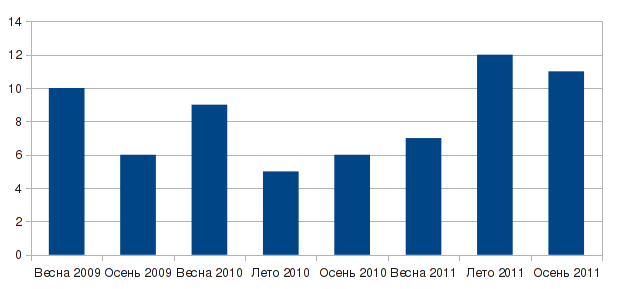
\includegraphics[width=1\textwidth]{01-projects.png}
    \caption{Число студенческих проектов по семестрам, 2009 - 2010 гг.}
    \label{projects}
  \end{center}
\end{figure}

Интересно также то, что в осенние семестры студенческие проекты оказывались менее популярны, чем в весенние. Это объясняется в большей степени тем, что весной для второкурсников происходит распределение по кафедрам, а активным участием в студпроекте можно заработать рекомендацию на интересующую кафедру. 

Сильный всплеск числа летних школ по программированию в 2011 году объясняется тем, что в организации этого мероприятия приняло участие сразу несколько компаний. Так, помимо традиционных проектов от ЗАО "Ланит-Терком", работа проводилась еще в двух направлениях: разработка дружественных пользовательских интерфейсов (при поддержке лаборатории Sprint и компании Intel), системному программированию и компьютерной безопасности (при поддержке следующих компаний -- Digital Design, EMC, Лаборатория Касперского, ЦентрИнформ). В этом году три этих направления были объединены в школу системного программирования при кафедре системного программирования СПбГУ. Однако, де-факто они были в значительной степени обособлены. В дальнейшем планируется теснее интегрировать между собой эти и другие летние IT-мероприятия для студентов, проводимые в СПбГУ.

\section{Проекты}

Остановимся подробнее на проектах, проведенных кафедрой системного программирования СПбГУ в 2011 году при сотрудничестве с ЗАО ``Ланит-Терком''. Большая часть из них была нацелена на изучение популярных сейчас мобильных и Интернет-технологий.

Так, несколько проектов было посвящено мобильной платформе Android. В рамках проекта ``Цена денег'' был разработан виджет, позволяющий отображать текущую ситуацию на различных рынках: российском валютном рынке, рынке цветных металлов и т.п. Другой проект ``Android-GeoCacheing.su'' был посвящен взаимодействию мобильных приложений с Интернет-сервисами, а также программному использованию GPS- приемника и магнитного компаса для реализации навигационных приложений. Работа была организована таким образом, что участники проекта знакомились со всеми этапами промышленной разработки ПО, начиная от создания технического задания и заканчивая выпуском финальной версии и написанием документации. Разработка в этих проектах происходила на языке Java. 

Проект ``iPhoneCF'' также был направлен на разработку ПО в области мобильных платформ. Его целью была создание инструмента для построения распределенных систем, работающих в операционной системе iPhone. Помимо, собственно, технологических вопросов (знакомство с операционными системами Mac OS, iPhone OS, а также языком Objective C и средой разработки Xcode) в данном проекте много внимания уделялось организации процесса разработки: работа велась в соответствии с ``гибкой'' методологией Scrum. В дальнейшем проект был продолжен под названием ``NeuronIOS'' и был посвящен созданию среды для реализации приложений для операционной системы iPhone, использующих аппарат нейронных сетей для обработки и анализа данных.

Проект ``Basis'' ставил своей целью создание среды для разработки php-приложений. Подобный инструментарий должен минимизировать затраты php-программиста на написание типовых управляющих элементов интерфейса и функций, а также предоставить разработчику каркас приложения, в котором разделена логика по обработке запросов, по работе с базой данных и т.п. Работы велись на языке PHP5 с использованием технологии AJAX.

Проект ``News Aggregating Agent'' предполагал создание приложения для социальных сетей, выполняющих просмотр собираемых с различных Интернет-источников новостей с возможностью фильтрации (по каналу, теме и/или дате). В рамках данного проекта студенты знакомились с программными интерфейсами ведущих социальных сетей и учились создавать Web-приложения на языке haXe.

Проект ``BoardGameMaster'' был посвящен другому популярному в наше время типу Интернет-приложений -- многопользовательским онлайн-играм. Задача данного проекта заключалась в разработке Web-сервиса, обеспечивающего возможность реализации любой игры с последовательными действиями игроков (от традиционных шахмат до современных настольных игр). В качестве примера клиентского приложения была разработана электронная версия настольной игры Dominion, разработка которого велась с использованием технологии Flash. Данный студпроект разрабатывался  в течение нескольких семестров.

В рамках проекта ``SUGAR'' студенты занимались созданием приложения для работы с кулинарными рецептами. Данное приложение позволяло по заданному набору продуктов выдать рекомендации, что их них лучше приготовить и как именно, а также подсказывало, что и в каком количестве необходимо дополнительно купить, предоставляя возможность осуществить заказ в Интернет-магазине. Здесь активно использовались технологии компании Miscrosoft -- платформа .NET 3.5-4, Silverlight, SQL Server.

Еще один проект проводился в контексте совместной инициативы ЗАО "Ланит-Терком" 
и кафедры системного программирования под названием 
DocLine~\cite{docLine1, docLine3, docLine2} и был направлен на освоение одной 
из самых популярных платформ разработки Java-приложений -- Eclipse, в том 
числе технологий работы с XML-документами и одной из самых мощных на 
сегодняшний день платформы для автоматизированного создания графических редакторов -- Eclipse Graphical Modeling Framework (GMF). В качестве области для экспериментов проводилась разработка средства для создания и управления семейством пользовательской документации программного продукта. 
 
Также внимания заслуживают проекты Embox~\cite{embox} и QReal~\cite{qreal2, qreal3, qreal}, разрабатываемые как свободное программное обеспечение и традиционно предлагаемые в рамках студенческих проектов и летних школ. 

Проект Embox был направлен на создание переносимой  и конфигурируемой операционной системы реального времени для нужд встроенных приложений. Данная система применяется на всех стадиях разработки -- от проектирования аппаратной части до создания функционального ПО. Операционная система  должна запускаться на различных процессорных архитектурах и включать в себя сетевой стек, файловую подсистему, частично поддержан стандарт POSIX и многое другое. Проект ведется уже несколько лет и каждый год привлекает много новых студентов, интересующихся внутренним устройством операционных систем.  

Проект QReal посвящен модельно-ориентированному подходу к разработке ПО, в частности, предметно-ориентированному моделированию -- созданию metaCASE-системы. В рамка проекта ведется разработка инструментария, позволяющего быстро разрабатывать новые графические языки и визуальные редакторы для них, а также генераторы кода в различные целевые языки, визуальные отладчики и другие полезные для разработки ПО средства. Студенты знакомятся с устройством визуальных языков, а также принимают активное участие в развитии системы QReal.


\section{Чему и как студенты учатся по время студенческих проектов и летних школ}

Обсудим в деталях, что студенты получают при участии в летних школах и студенческих проектах такого, чего они обычно не могут получить при традиционном университетском образовании.

Прежде всего, это знакомство с новейшими технологиями программирования и передовыми областями индустрии. Чтобы оставаться конкурентоспособными на рынке, компании следят за последними тенденциями и новейшими направлениях, критичными для их бизнеса, и стараются поддерживать у своих сотрудников соответствующие компетенции на высоком уровне. При этом чем более новым является тот или иной язык программирования, инструментарий или технология, тем меньше по ним доступно учебных материалов. Таким образом, непосредственное общение с носителями этих знаний из индустрии становится, фактически, единственным достоверным источников информации для студентов, да и для университетских преподавателей.  
Еще одной особенностью проведения студпроектов является то, что студенты вольны сами выбирать проект для участия. При этом очень часто случается так, что изначально каждый вступает сразу в несколько проектов, из которых в течение некоторого времени выбирает наиболее интересный для себя (продуктивно работать в нескольких проектах и хорошо учиться практически никогда не получается). Это очень важно, поскольку студенты, особенно на первом-втором курсах, не всегда знают, что они хотят, и чем у них получится заниматься, что выбрать для себя из огромного числа возможных направлений в программной инженерии. В такой ситуации для студента было бы идеальным попробовать свои силы в нескольких областях, прежде чем этот выбор нужно будет делать уже по-настоящему при устройстве на работу. В некотором смысле этому способствуют курсовые и дипломные работы, а также производственная преддипломная практика. Однако курсовые работы часто имеют более научную и  исследовательскую направленность, чем производственную, а производственную практику студент проходит уже в самом конце обучения. Наличие разнообразных проектов уже на младших курсах обучения видится нам удачным средством для формирования у студентов кругозора, поэтому мы всячески заинтересованы в расширении спектра наших проектов. 

В студенческих проектах есть возможность непосредственного обучения инженерным практикам, ставшими де-факто обязательной частью повседневной работы промышленного программиста -- средствами тестирования, документирования, конфигурационного управления и др. Так, например, на ``игрушечных'' учебных заданиях, которые предлагаются на лабораторных и практичесвких занятиях в рамках стандартного учебного процесса и которые редко превышают нескольких тысяч строк кода, студенту сложно понять, зачем ему может понадобится осуществлять ночные сборки и регулярно проводить регрессионное тестирование. Зачем и в каком объеме нужно разрабатывать модульные тесты? Почему в системе отслеживания ошибок (bugtracking system) полезно иметь возможность назначить ошибку конкретному разработчику и уметь связывать ошибку с изменениями в коде, исправляющими эту ошибку? Как зависит организация процесса разработки ПО от выбранной политики создания ветвей (branching policy) в современных системах версионного контроля кода? На эти и многие другие актуальные в наше время вопросы сложно ответить, сидя за партой, их нужно постичь на собственном опыте. Только тогда приходит осознание необходимости использования тех или иных инструментальных средств, и того, как их нужно правильно применять. И это -- путь формирования производственной культуры. Отсутствие глубокого понимания таких вопросов приводит к тому, что инструменты применяются не вследствие того, что они нужны в данной конкретной ситуации, а потому, что ``так научили'' или ``так принято''~\cite{cargoCult}. Участие в студенческих проектах дает студентам возможность познакомиться с различными инженерными практиками гораздо в более реальных условиях, не принимая ничего на веру. 

Стоит также отметить, что часто к нам приходят и студенты со смежных специальностей (иногда даже не IT-профиля), активно стремящиеся познакомиться с промышленным программированием самостоятельно. Не имея даже университетских занятий по программной инженерии, участие в студенческих проектах становится для них существенной подготовкой перед реальной работой в промышленных компаниях.

Еще один важный навык, которому можно обучиться лишь на практике -- умение общаться. Здесь речь идет как о живом общении, так и о культуре производственного сетевого общения.  Очень важно уметь продуктивно работать в команде, в частности, уметь задавать вопросы и прояснять для себя неясные моменты в постановке задачи, а не домысливать их самому (эта привычка студентов на мат.-мех. факультете очень сильна в силу акцента на аналитическом, подходе к решению задач, но она приводит к тому, что они часто начинают делать что-то совершенно свое, отличное от исходного задания). Также важно уметь рассказать о своей работе самым разным людям -- начальству, товарищам, независимым экспертам (как упоминалось ранее, в конце года проводится презентация результатов работы по каждому студенческому проекту, на которую приглашаются все желающие, и объявления о которой расклеиваются по всему факультету заранее). Внутренние и внешние коммуникации являются важной частью повседневной жизни любого проекта, и этому студентов тоже нужно учить. При этом можно прочитать все книги по ораторскому искусству, но публично выступать от этого вряд ли кто-то сможет научиться без реальной практики. Важна также культура производственного сетевого общения (у нас этому начинают учить студентов с первой встречи по проекту): на письма нужно отвечать, и делать это оперативно, адекватно заполнять поле с темой письма, не посылать писем только со вложением и с пустым "телом" и многое другое. Отсутствие этой, казалось бы, элементарной культуры общения будет не только вносить неприятные моменты в общение между членами команды, но и может сильно испортить внешнюю репутацию компании при общении с заказчиками.

Важной особенность организации рабочего процесса в промышленных компаниях, является дисциплина обязательств~\cite{ obyzat}:
\begin{itemize}
 \item готовность работников принимать на себя обязательства перед другими;
 \item четкое определение тех обязательств, которые они на себя берут;
 \item стремление прилагать должные усилия к выполнению своих обязательств;
 \item готовность честно и незамедлительно информировать об угрозах выполнению своих обязательств и т.п.
\end{itemize}
Отсутствие подобной дисциплины является неприемлемым для промышленности. Однако, в университетах традиционно складываются более демократичные порядки -- зачастую считается допустимым опоздать на занятие, многие студенты позволяют себе задерживать результаты по курсовым работам, исчезать и появляться в течение семестра, наивно надеясь все сдать в последний момент или, на крайний случай, в начале следующего семестра и т.п. Проведение студенческих проектов помогает воспитать в студентах чувство ответственности за свою работу, осознание важности не терять связь с руководителем и коллегами, брать на себя обязательства и не подводить своих коллег, следовать общему процессу.

\section{Выводы} 

Традиционное университетское образование направлено в первую очередь не на получение практических навыков, а на формирование особого образа мышления студентов -- умения искать и анализировать информацию, находить новые пути решения. Для обучения по специальностям, связанным с программной инженерией, это имеет свои плюсы и минусы: с одной стороны, выпускник классического университета получает фундаментальную теоретическую подготовку для работы в своей области -- знает основные алгоритмы и структуры данных, языки программирования, технологии и подходы к разработке ПО и т.д. С другой стороны, на лицо явный недостаток практических навыков, и это хорошо понимают в промышленных компаниях -- к большинству из открытых в индустрии вакансий ставится требованием наличие нескольких лет опыта работы по специальности. Осознавая это, студенты IT-специальностей, начиная с третьего-четвертого курса, уже пытаются устраиваться на работу стажерами. Но очень часто это приводит тому, что у них остается очень мало времени на учебу. В результате уровень получаемого выпускниками образования снижается.

Решать эту проблему, безусловно, нужно. А так как речь идет о практической дисциплине, то большую роль в формировании профессиональных навыков программной инженерии играет передача опыта, описание типичных ошибок и практик, зарекомендовавших себя в индустрии, примеры выполнения реальных проектов и т.п. Ведь нельзя стать хорошим программистом, только лишь читая книги, сидя в лекционном зале или в компьютерном классе. 

Одной из форм получения реального промышленного опыта наиболее гармоничным образом является совместная (промышленные компании и университеты) организация студенческих проектов и летних школ. Участвуя в подобных проектах, студенты не только повышают свои навыки программирования, но и знакомятся с полезными инженерными практиками, которые помогут им по завершении обучения быть полноценными специалистами в области программной инженерии. Так, студенты учатся взаимодействовать в команде, использовать системы версионного контроля для кода и документации, выявлять и анализировать требования, оценивать и планировать задачи, участвовать в ревью кода, архитектуры, документации и других артефактов проекта. Кроме того, в рамках студпроекта студент может подготовить курсовую работу, а также получить рекомендацию для устройства на работу в компанию, которую представляет руководитель проекта. 

В настоящее время при организации студенческих проектов и летних школ можно столкнуться с множеством сложностей на самых разных уровнях. 

\begin{itemize}
 \item Финансирование. Идеальным является совместные финансовые вложения бизнес-компаний и университетов. Также можно привлекать различные гранты, фонды на региональном, федеральном и международном уровнях. 
 \item Формальные вопросы с университетом, включая организацию подходящих для работы помещений. Сложность и трудоемкость этой деятельности нельзя приуменьшать, так как российские университеты все строже регламентируют свою деятельность, и необходимо получить множество различных разрешений и одобрений, попасть в различные планы официальных мероприятий и т.д. 
 \item Привлечение заинтересованных в IT-компаниях специалистов для руководства проектами. При  этом идеальной является ситуация, когда специалистам в университете интересна тематика того или иного студенческого проекта, и они помогают наладить долгосрочное сотрудничество с промышленной компанией и гармоничный учебный процесс для студентов.  
 \item Интересные задачи. Для летних школ и студенческих проектов необходимо подобрать подходящие задачи, которые заинтересуют студентов и будут актуальными для современной программной инженерии, а также будут им посильны. 
 \item Методики проведения студенческих проектов и летних школ. Данные методики должны  позволить проводить школы и проекты максимально эффективными -- при этом есть много нюансов, которые будут отличаться в каждом конкретном случае.  
 \item Хороший сайт, в особенности, если студенческая школа проводится регулярно. Это крайне полезно для привлечения студентов, компаний-участников и финансирования. 
\end{itemize}
  
Как показывает опыт проведения таких мероприятий на базе кафедры системного программирования СПбГУ, для студентов опыт участия в них крайне полезен. И растущее с каждым годом число проводимых по всему миру летних школ по программированию и информатике лишь подтверждает это.

\begin{thebibliography}{9001}

  \bibitem{brooks} Ф. Брукс. Мифический человеко-месяц или Как создаются программные системы, Символ-Плюс, СПб., 2011.
  \bibitem{gagarsky} Р.К Гагарский. Программа подготовки специалистов в IT-компании // Системное программирование. Вып. 3. СПб.: Изд-во СПбГУ. 2008, С. 141-156.
  \bibitem{tercom} ЗАО ``Ланит-Терком'', \url{www.lanit-trecom.ru}
  \bibitem{apkit} Квалификационные требования (профессиональный стандарт) в области информационных технологий по специальности ``Программист'', \url{http://apkit.ru/files/programer.doc}
  \bibitem{saratov} Я.А. Кириленко. Разработка свободного программного обеспечения для школ как средство обучения программной инженерии // Материалы IX Всероссийской конференции <Преподавание информационных технологий в Российской Федерации>. Саратов. 2011.
  \bibitem{docLine1} Д.В.Кознов, К.Ю.Романовский.  DocLine: метод разработки документации семейства программных продуктов. Программирование, 2008, № 4 С. 1-13.
  \bibitem{obyzat} Д.В.Кознов. Введение в программную инженерию, часть I. Учебное пособие. СПбГУ. 2005. 41 с. 
  \bibitem{qreal2} Кузенкова А.С., Дерипаска А.О., Таран К.С., Подкопаев А.В., Литвинов Ю.В., Брыксин Т.А., Средства быстрой разработки предметно-ориентированных решений в metaCASE-средстве QReal // Научно-технические ведомости СПбГПУ, Информатика, телекоммуникации, управление. Вып. 4 (128). СПб.: Изд-во Политехнического Университета. 2011. С. 142-145.

  \bibitem{intel1} Летняя школа Intel 2010, \url{http://software.intel.com/ru-ru/articles/summer-school-2010-main/}
  \bibitem{intel2} Летняя школа Intel 2011, \url{http://software.intel.com/ru-ru/articles/summer-school-2011/}

  \bibitem{qreal3}Осечкина М.С., Брыксин Т.А., Литвинов Ю.В., Кириленко Я.М. Поддержка жестов мышью в мета-CASE-системах // Системное программирование. Вып. 5: Сб. статей / Под ред. А.Н.Терехова, Д.Ю.Булычева.  СПб.: Изд-во СПбГУ, 2010. С. 52-75.
  \bibitem{curriculum} Рекоммендациях по преподаванию программной инженерии и информатики в университетах, \url{http://www.intuit.ru/research/se2004.pdf}
  \bibitem{docLine3}К.Ю.Романовский, Д.В.Кознов. Язык DRL для проектирования и разработки документации семейства программных продуктов // Вестник Санкт-петербургского университета, Серия 10, Информатика, № 4, 2007. С. 110-122.
  \bibitem{embox} Проект Embox, \url{http://code.google.com/p/embox/}
  \bibitem{school9} Семинары компании SoSE, Саариселка, Финляндия, \url{http://www.cs.tut.fi/~sose/index_files/Page1211.htm}
  \bibitem{docLine2}Смирнов М.Н., Кознов Д. В., Дорохов В. А., Романовский К.Ю.  Программная среда WebMLDoc для автоматизированного отслеживания изменений в пользовательской документации Web-приложений // Сб. Системное программирование./ Вып. 5, под ред. А.Н.Терехова и Д.Ю.Булычева. СПб.: Изд. СПбГУ, 2010. C. 32-51.
  \bibitem{intel3} Студенческие школы компании Intel, \url{http://www.intel.com/cd/corporate/education/emea/rus/highered/student/398668.htm}
  \bibitem{schoolList} Список  евпропейских летних школ с 1998 по 2011 по IT, \url{http://user.it.uu.se/~bengt/Info/summer-schools.shtml}
  \bibitem{school7} Школа, посвященная вопросам многоядерных архитектур, Амстердам, Голландия, 2011, \url{http://www.multimoore.nl/}
  \bibitem{qreal} Терехов А.Н., Брыксин Т.А., Литвинов Ю.В., Смирнов К.К., Никандров  Г.А., Иванов В.Ю., Такун Е.И. Архитектура среды визуального  моделирования QReal // Системное программирование. Вып. 4: Сб. статей  / Под ред. А.Н.Терехова, Д.Ю.Булычева. 2009. С. 171-196.



  \bibitem{school3} Coupled Software Transformations Workshop, Брага, Португалия, 2011, \url{http://www.di.univaq.it/CSXW2011/}
  \bibitem{school1} 8th LASER Summer School on Software Engineering, о. Эльба, Италия, 2011, \url{http://laser.inf.ethz.ch/2011/}
  \bibitem{school5} 8th International Summer School on Software Engineering, Салермо, Италия, 2011, \url{http://www.sesa.dmi.unisa.it/seschool/}
  \bibitem{school2} 4th Summer School on Generative and Transformational Techniques in Software Engineeringh, Брага, Португалия, 2011,  \url{http://gttse.wikidot.com/}
  \bibitem{school10} Finnish-Russian University Cooperation in Telecommunications, \url{http://www.fruct.org/}
  \bibitem{swebok} Guide to the Software Engineering Body of Knowledge (SWEBOK), \url{http://www.computer.org/portal/web/swebok}
  \bibitem{google} Google Summer of Code, \url{http://code.google.com/intl/ru-RU/soc/}
  \bibitem{langList} HOPL: an Interactive Roster of Programming Languages,  \url{http://hopl.murdoch.edu.au/}
  \bibitem{school4} Industry Track of Software Language Engineering, Брага, Португалия, 2011, \url{http://planet-sl.org/itsle2011/index.php?option=com_content&view=article&id=128&Itemid=169}
  \bibitem{ms2} Microsoft Сomputer Vision School, Moscow, 2011, \url{http://summerschool2011.graphicon.ru/en}
  \bibitem{ms3} Microsoft Data Structures and Algorithms School, St.Petersburg, 2010, \url{http://logic.pdmi.ras.ru/midas/en/about}
  \bibitem{school8} PRACE Summer School, Эспоо, Финляндия, 2011, \url{http://www.csc.fi/english/csc/courses/archive/summerschool2011}
  \bibitem{school6} Programming Languages for Concurrent \& Parallel Computing, Стокгольм, Швеция, 2011, \url{http://www.it.uu.se/research/upmarc/events/SS2011/Start.html}
  \bibitem{cargoCult} Steve McConnell, Cargo Cult Software Engineering. From the Editor, IEEE Software, March/April 2000, \url{http://stevemcconnell.com/ieeesoftware/eic10.htm}
  \bibitem{ms1} Summer School in Software Engineering and Verification, Moscow, 2011, \url{http://research.microsoft.com/en-us/um/redmond/events/sssev2011/}


\end{thebibliography}

\end{document}
